\documentclass[twocolumn]{article}
\usepackage{ctex}
\usepackage{amsmath}
\usepackage{amsfonts}
\usepackage{amssymb}
\usepackage{graphicx}
\usepackage{float}
\usepackage{listings}
\usepackage{color}
\usepackage{geometry}
\usepackage{fancyhdr}
\usepackage{titlesec}
\usepackage{tikz}
\usepackage{pgfplots}
\usepackage{pgfplotstable}
\usepackage{booktabs}
\usepackage{caption}
\usepackage{subcaption}
\usepackage{algorithm}
\usepackage{algorithmic}
\usepackage{multirow}
\usepackage{array}
\usepackage{enumitem}
\usepackage{hyperref}
\usepackage{svg}

\title{LAMP: Large-language-model Augmented Mobile Testing Path Exploration Based on Kea}

\author{Group 07 \\ 李鹏达, 武泽恺, 张耘彪}
\date{}

\begin{document}

\maketitle

\section{背景}

移动应用自动化测试是目前正在快速发展的领域,研究热点包括UI引导的测试输入生成、基于属性的
测试(PBT)、大语言模型(LLM)的应用以及上下文感知的文本输入生成等技术方向。DroidBot\cite{li2017droidbot}等UI引导的测试
工具通过动态构建状态转移模型,生成高效的测试输入,适用于兼容性测试和安全分析;
基于属性的测试\cite{xiong2024general}通过定义功能属性并生成输入事件序列,有效检测非崩溃性功能错误;
InputBlaster\cite{liu2024testing}, QTypist\cite{liu2023fill} 和 GPTDroid\cite{liu2024make} 等工具利用大语言模型的语义理解和生成能力,在异常输入生成、文本输入生成、测试脚本生成和Bug复现等方面表现出色,显著提升了测试覆盖率和错误检测能力;上下
文感知的文本输入生成技术\cite{liu2023fill}则通过提取GUI上下文信息,生成符合语义的输入,填补了文本输入测试的
空白。这些技术在移动应用测试中取得了显著的进展。

其中, Kea\cite{xiong2024general}是一个基于属性测试的移动应用测试工具。它将基于属性的测试引入移动应用测试,通过定义功能属性并结合路径探索,发现Android应用中的非崩溃性功能错误,提供了更深入的功能验证能力。


Kea 目前提供了三种路径探索策略:随机探索、主路径引导探索、和大语言模型辅助的探索。其中,随机探索策略随机地生成输入事件序列,主路经引导探索策略在用户指定的应用``主路径''附近进行随机探索。
而大语言模型引导策略则是对随机策略的加强——它在随机探索的基础上,检测当前是否处于UI陷阱(``焦油坑''\cite{khan2024aurora})。若处于UI陷阱,则使用大语言模型生成输入事件,试图跳出UI陷阱。
然而,Kea 现有的大语言模型引导策略仍存在一些不足,可以得到进一步加强。

\section{问题}

现有的大模型引导策略(LLM策略)主要分为相似度检测和生成事件两个模块。图 \ref{fig:llm} 展示了现有的大模型引导策略的基本流程。

进行相似度检测时,主要使用 OpenCV 对比两个UI状态的屏幕截图,从而计算两个状态之间的相似度,当连续多次相似度超过设定的阈值时,Kea 认为当前处于UI陷阱。此时,Kea 会使用大语言模型生成输入事件,试图跳出UI陷阱。
基于现有的UI状态信息和可能的输入事件,Kea 会询问大语言模型,由大语言模型给出一个输入事件并执行。

\begin{figure}
    \centering
    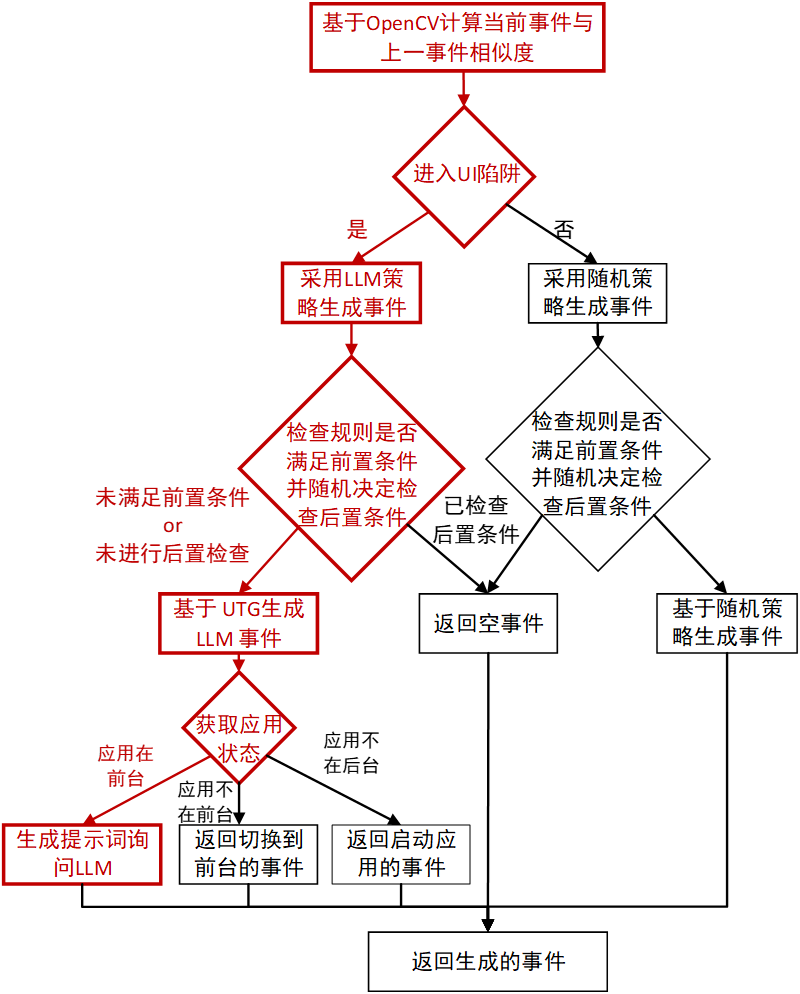
\includegraphics[width=0.5\textwidth]{img/llm.png}
    \caption{Kea现有的大模型引导策略示意图}
    \label{fig:llm}
\end{figure}

\begin{figure}
    \centering
    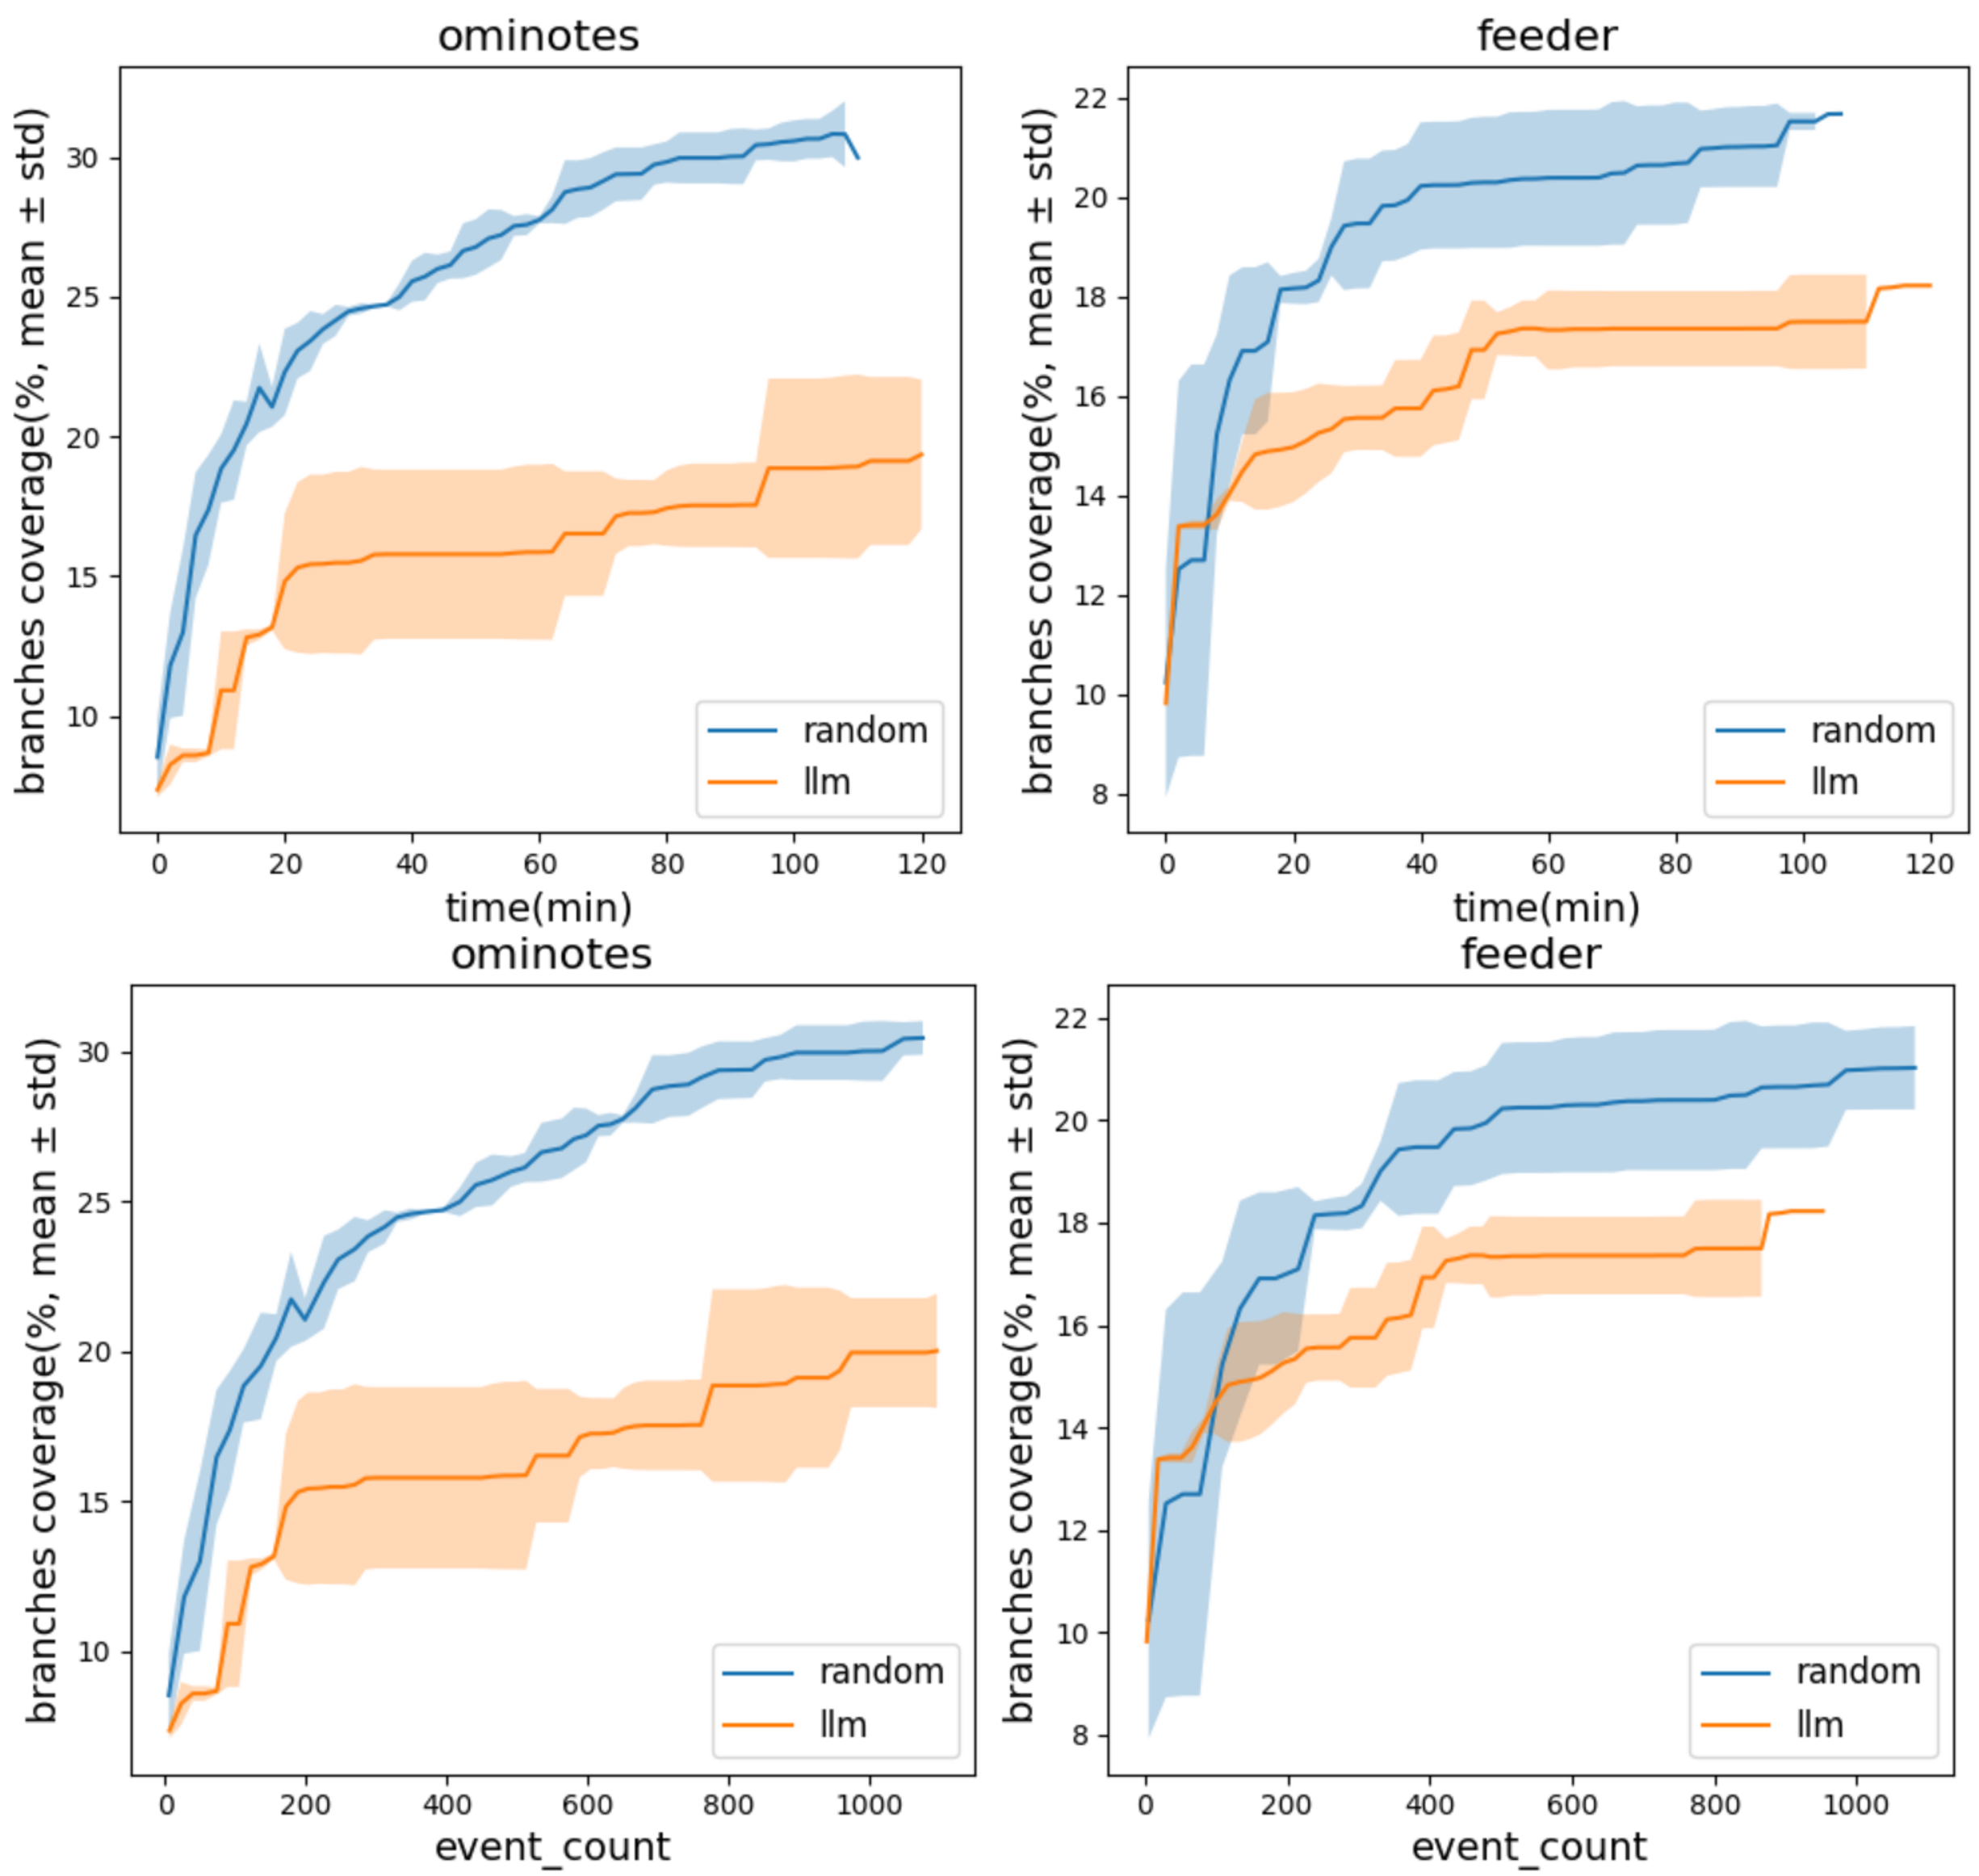
\includegraphics[width=0.5\textwidth]{img/llm_test.png}
    \caption{LLM策略和随机策略相同时间或相同事件数量时代码分支覆盖率}
    \label{fig:llm_test}
\end{figure}

然而,现有LLM策略效果不佳。图 \ref{fig:llm_test} 展示了运行LLM策略和随机策略相同时间或相同事件数量时的代码分支覆盖率,LLM策略相比随机策略不但没有提升,甚至有所下降。

这向我们揭示了现有策略存在的一些问题:1) LLM 策略在解决 UI 陷阱方面效果不佳,原因在于其生成的事件不准确,且缺乏上下文感知能力;2) LLM 策略由于需要频繁调用,会产生显著的运行开销;3) 现有的相似度检测方法可能会导致误判。

因此,我们提出了一种新的大语言模型辅助的路径探索策略,称为LAMP(Large-language-model Augmented Mobile Testing Path Exploration Based on Kea)。LAMP 通过引入基于语义的UI陷阱检测算法和基于迭代事件序列生成 的增强型LLM探索策略,结合大语言模型的语义理解和生成能力,提升了路径探索的效率和准确性。

我们希望 LAMP 能解决以下问题:
1) 提高UI陷阱检测的准确性,减少误判;2) 平衡大语言模型的调用频率,减少运行开销;3) 提升生成事件的准确性和上下文感知能力。

\section{方法}

\subsection{基于语义的UI陷阱检测算法}


\bibliographystyle{IEEEtran}
\bibliography{ref}

\end{document}